\subsection{Builder}
Viene utilizzato per separare la logica di costruzione di un oggetto complesso dalla sua rappresentazione. Permette inoltre di creare dinamicamente dei nuovi oggetti mediante degli algoritmi di creazione che sono facilmente intercambiabili tra loro.

\begin{figure}[ht]
    \centering
    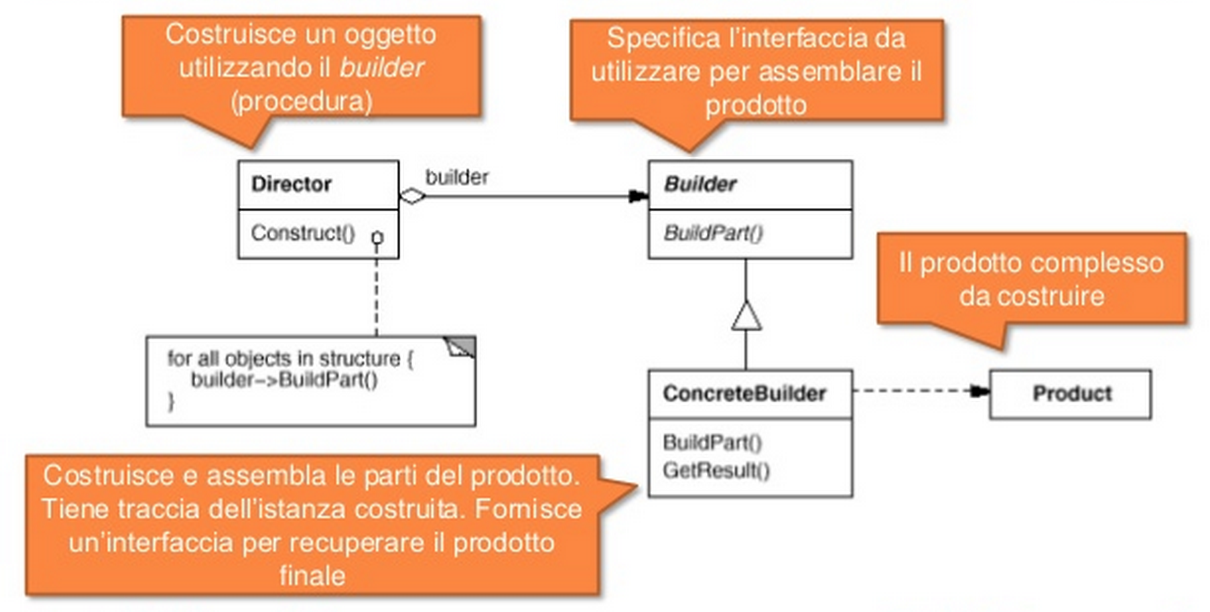
\includegraphics[width=0.8\textwidth]{immagini/builder.png}
    \caption{Builder}
\end{figure}
\FloatBarrier

In questo modo viene isolato il codice di costruzione dell'oggetto, rendendolo più facile da estendere senza far esplodere il numero di parametri da passare al costruttore (telescoping).
Inoltre, se vengono aggiunti campi, non è necessario andare a modificare il codice del client, ma le modifiche vengono limitate al director.
\subsubsection{Utilizzo}
\begin{enumerate}
\item Il client crea un builder per l'oggetto che deve costruire;
\item Il client crea un director passandogli il builder con cui costruire l'oggetto;
\item Il director crea l'oggetto finale utilizzando i vari metodi messi a disposizione dal builder;
\item Il client ottiene il riferimento all'oggetto finale.
\end{enumerate}
\begin{figure}[ht]
    \centering
    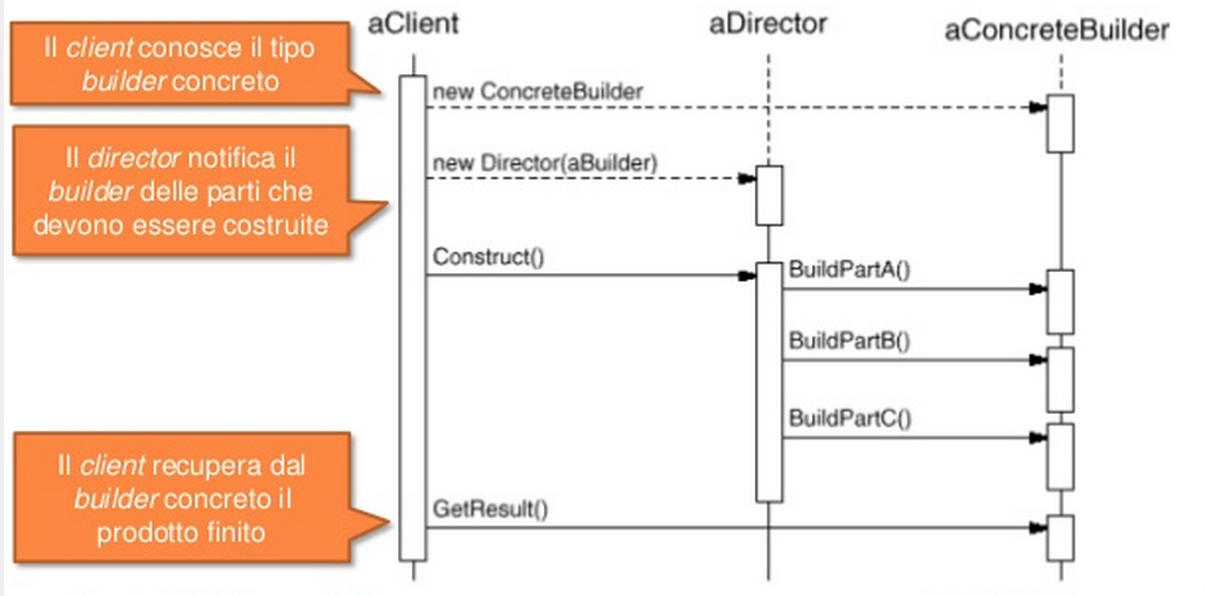
\includegraphics[width=0.8\textwidth]{immagini/builderSequence.png}
    \caption{Diagramma di sequenza di un builder}
\end{figure}
\FloatBarrier
